\documentclass[]{article}
\usepackage{amsmath,amssymb,amsthm}
\usepackage[utf8]{inputenc}
\usepackage{lmodern}
%\usepackage{circuitikz}
\makeatletter
\@ifpackageloaded{tex4ht}{
    \def\pgfsysdriver{pgfsys-tex4ht.def}
}
\makeatother
\usepackage{pgfplots}
\usepackage{pgfplotstable}
\usepackage{pgf,tikz}
\usetikzlibrary{shapes,backgrounds,positioning,matrix,decorations}

\usepackage{siunitx}
\usepackage{python}
\usepackage{ifxetex,ifluatex}
\usepackage{listings}
% \usepackage[xindy,acronym,nomain,toc]{glossaries}
% \makeglossaries
%\usepackage[xindy]{imakeidx}
%\makeindex
\setlength{\parskip}{3mm}
\newtheorem{axiom}{Axiom}
\newtheorem{definition}{Definition}
\newtheorem{comment}{Comment}
\newtheorem{example}{Example}
\newtheorem{lemma}{Lemma}
\newtheorem{property}{Property}
\newtheorem{problem}{Problem}
\newtheorem{remark}{Remark}
\newtheorem{theorem}{Theorem}
\newtheorem{script}{Script}

\usepackage{fixltx2e} % provides \textsubscript
% use upquote if available, for straight quotes in verbatim environments
\IfFileExists{upquote.sty}{\usepackage{upquote}}{}
\ifnum 0\ifxetex 1\fi\ifluatex 1\fi=0 % if pdftex
  \usepackage[utf8]{inputenc}
\else % if luatex or xelatex
  \ifxetex
    \usepackage{mathspec}
    \usepackage{xltxtra,xunicode}
  \else
    \usepackage{fontspec}
  \fi
  \defaultfontfeatures{Mapping=tex-text,Scale=MatchLowercase}
  \newcommand{\euro}{€}
\fi
% use microtype if available
\IfFileExists{microtype.sty}{\usepackage{microtype}}{}
\usepackage{graphicx}
% Redefine \includegraphics so that, unless explicit options are
% given, the image width will not exceed the width of the page.
% Images get their normal width if they fit onto the page, but
% are scaled down if they would overflow the margins.
\makeatletter
\def\ScaleIfNeeded{%
  \ifdim\Gin@nat@width>\linewidth
    \linewidth
  \else
    \Gin@nat@width
  \fi
}
\makeatother
\let\Oldincludegraphics\includegraphics
{%
 \catcode`\@=11\relax%
 \gdef\includegraphics{\@ifnextchar[{\Oldincludegraphics}{\Oldincludegraphics[width=\ScaleIfNeeded]}}%
}%
\ifxetex
  \usepackage[setpagesize=false, % page size defined by xetex
              unicode=false, % unicode breaks when used with xetex
              xetex]{hyperref}
\else
  \usepackage[unicode=true]{hyperref}
\fi
\hypersetup{breaklinks=true,
            bookmarks=true,
            pdfauthor={Dilawar Singh},
            pdftitle={Problem 2},
            colorlinks=true,
            citecolor=blue,
            urlcolor=blue,
            linkcolor=magenta,
            pdfborder={0 0 0}}
\urlstyle{same}  % don't use monospace font for urls
\setlength{\parindent}{0pt}
\setlength{\parskip}{6pt plus 2pt minus 1pt}
\setlength{\emergencystretch}{3em}  % prevent overfull lines
\setcounter{secnumdepth}{5}

\title{Problem 2}
\author{Dilawar Singh}
\date{A markdown version of this document is available \%
\href{http://github.com/dilawar/courses/raw/master/NeuroCourse/Assignments/Second/Problem02/L2_Q2_DilawarSingh.pandoc}{here}}

\begin{document}
\maketitle

\begin{problem}

    I apply a square wave current of baseline \SI{0}{pA} and max \SI{10}{pA} ,
    to a spherical cell with a capacitance of \SI{0.01}{F/m^2} and diameter
    \SI{10}{u}, and resting potential is \SI{-60}{mV}, $R_A = \SI{1}{\ohm m}$, and
    $R_M = \SI{1}{\ohm m^2}$ . Draw the waveform of the output for 2 full cycles of
    the stimulus, for a frequency of 10 Hz, 100 Hz, and 1000 Hz respectively.
    Your graph should be labelled with voltage and time axes.  I don’t need a
    word explanation, but you can put in your calculation if you like. Doesn’t
    have to be hugely precise, factor of 2 in the peak height is fine.  The
    graph shape matters too. I suggest you draw in pencil, and scan it in so you
    can upload as a pdf.

\end{problem}

The equivalent circuit of cell is in fig \ref{fig1}. But we should
convert a spherical cell to cylinderical first before we can use this
electrical equivalent. Lets assume that both cylinder and sphere has the
same volume and surface area. Let assume the radius of cylinder is $r'$
and its length is $l$ and the radius of sphrerical cell is $r$.

\begin{figure}[h]
    \centering
    \usetikzlibrary{shapes,shadows}
    \begin{tikzpicture}
        \shade[shading=ball, ball color=red!20] (0,0,0) circle (1cm);

        \draw [<->,thick] (1.5,0) -- +(2,0);
        \node[cylinder
        , cylinder uses custom fill
        , minimum width=1cm
        , minimum height=2.5cm 
        , cylinder body fill=red!25
        , cylinder end fill=red!50
        ] at (6,0)  {};
    \end{tikzpicture}
    \caption{A spherical cell and its equivalent cylinder}
    \label{fig1}
\end{figure}

\[ \frac{4}{3}{\pi r^3} = \pi r'^2 l \] \[ 4 \pi r^2 = 2 \pi r' l \]

This gives $r'=\frac{2}{3}r$ and $l=3r$. We dont have to calculate value
of $R_a$. Values of other parameters are following:

\begin{align}
    R_m &= \frac{R_M}{2 \pi r' l} = \frac{R_M}{100 \pi r^2 }  = 3.15 \times
    10^{9} \\
    C_m &= C_M 2\pi r' l = C_M 4\pi r^2 =  3.1416 \times 10^{-12} F
\end{align}

\begin{figure}[h]
    \usetikzlibrary{shapes,shadows,circuits.ee.IEC}
    \centering
    \begin{tikzpicture}[circuit ee IEC
        ]
        % Connect R_a
        \draw (-3,0) to[resistor={info={$R_a$}}] ++(3,0)
        ;
        \draw (0,0) -- ++(0,-0.5) -- ++(-1,0)
        to[resistor={info={$R_m$}}] ++(0,-2) 
        to[voltage source={direction info={<-,volt=0.06}}] ++(0,-1.5)
        ;
        \draw (0,0) -- ++(0,-0.5) -- ++(1,0)
        to[capacitor={info={$C_m$}}] ++(0,-3.5) -- ++(-2,0)
        ;
        \draw (0,-4.0) -- ++(0,-0.5) to[ground] ++(0,-0.5)
        ;
        %% Connect a probe to inject current 
        \draw  (2,1) to[current source={direction info={->,ampere=10p}}] ++(-1,0)
            -- ++(-1,-1) node [above] {$b$}
        ;
        \draw (2,1) -- ++(1,0) to[ground] ++(0.5,0)
        ;

    \end{tikzpicture}

    \caption{Injecting current into cell. Axial resistance $R_a$ is useless now.
    We measure voltage at node $b$ when current is being injected into cell.}
    \label{fig:sphere}
\end{figure}

\subsection{Waveform}\label{waveform}

The peak value will remain -0.060 V of waveform. The resistor will be
charged through $R_m$ and the time constant $\tau$ of charging is
$R_m \times C_m = 0.01$ s. In this time, the waveform get's $63 \%$ of
peak value i.e. $- 60 + 31.5 = - 29.5$ mV. Following is spice netlist
for this circuit the waveforms. These spice scripts can be found
\href{http://github.com/dilawar/courses/raw/master/NeuroCourse/Assignments/Second/}{here}

\begin{figure}[htbp]
\centering
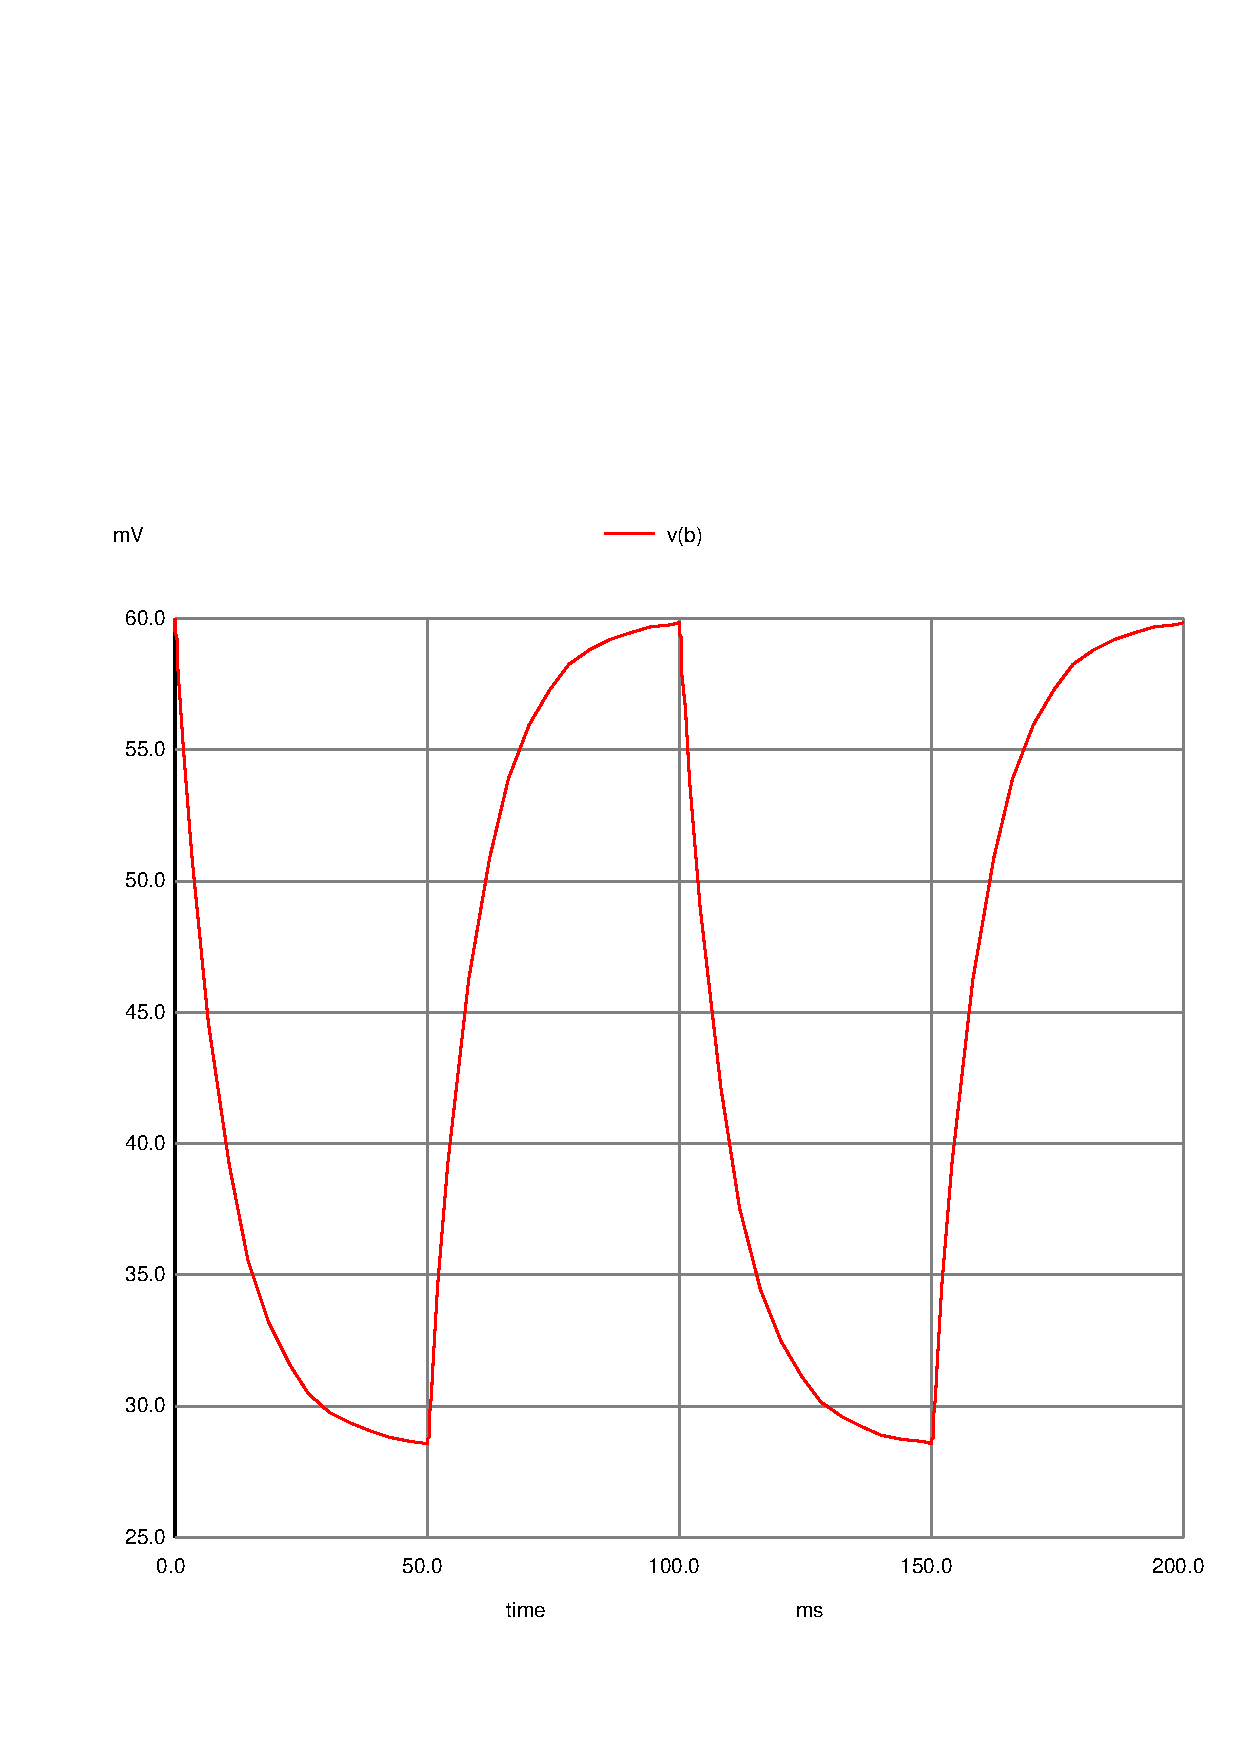
\includegraphics{./plot_10hz.pdf}
\caption{Waveform when 10Hz pulse is applied Since charging and
discharging is happening through same path, we see a symmetry.}
\end{figure}

\begin{figure}[htbp]
\centering
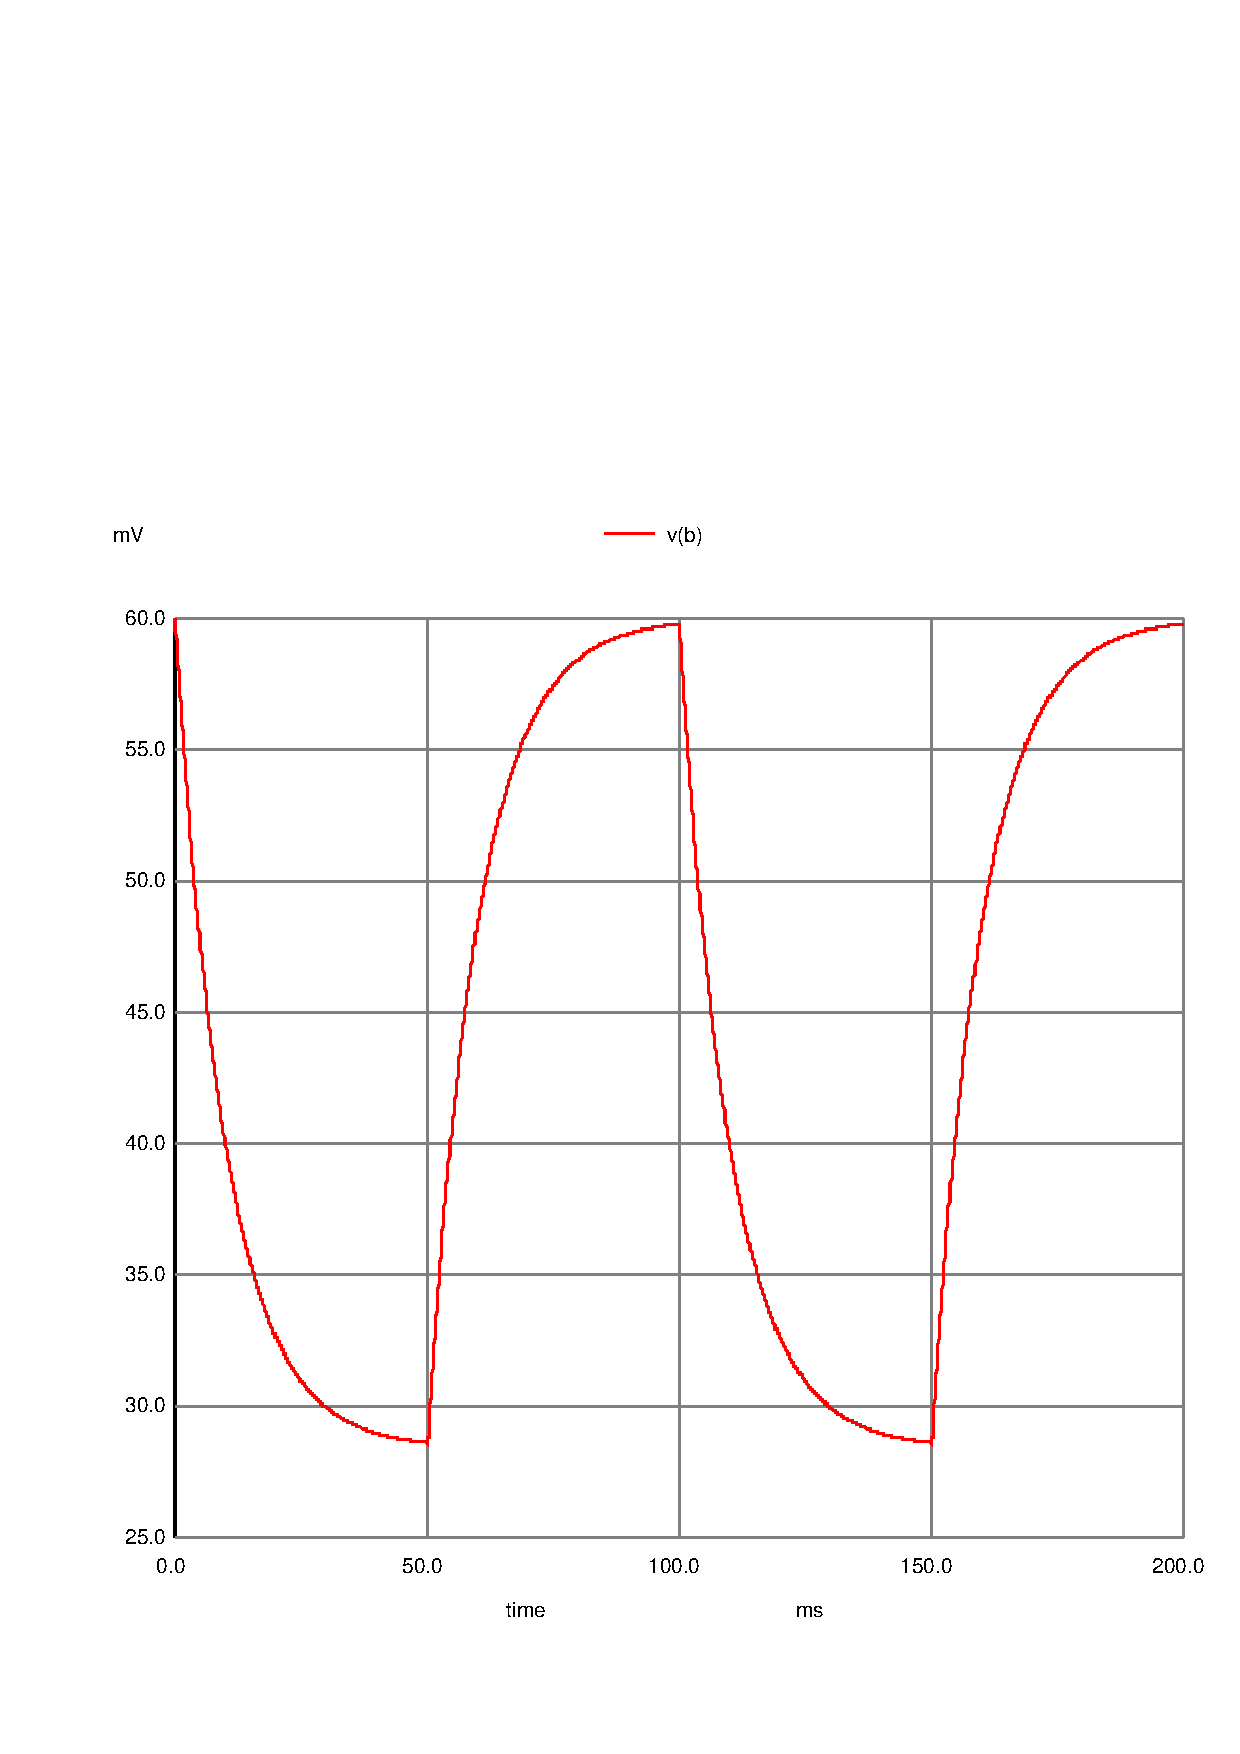
\includegraphics{./plot_100hz.pdf}
\caption{20 pulse of 100 Hz pulse are applied. Discharging starts before
capacitor is fully charged and vice versa.}
\end{figure}

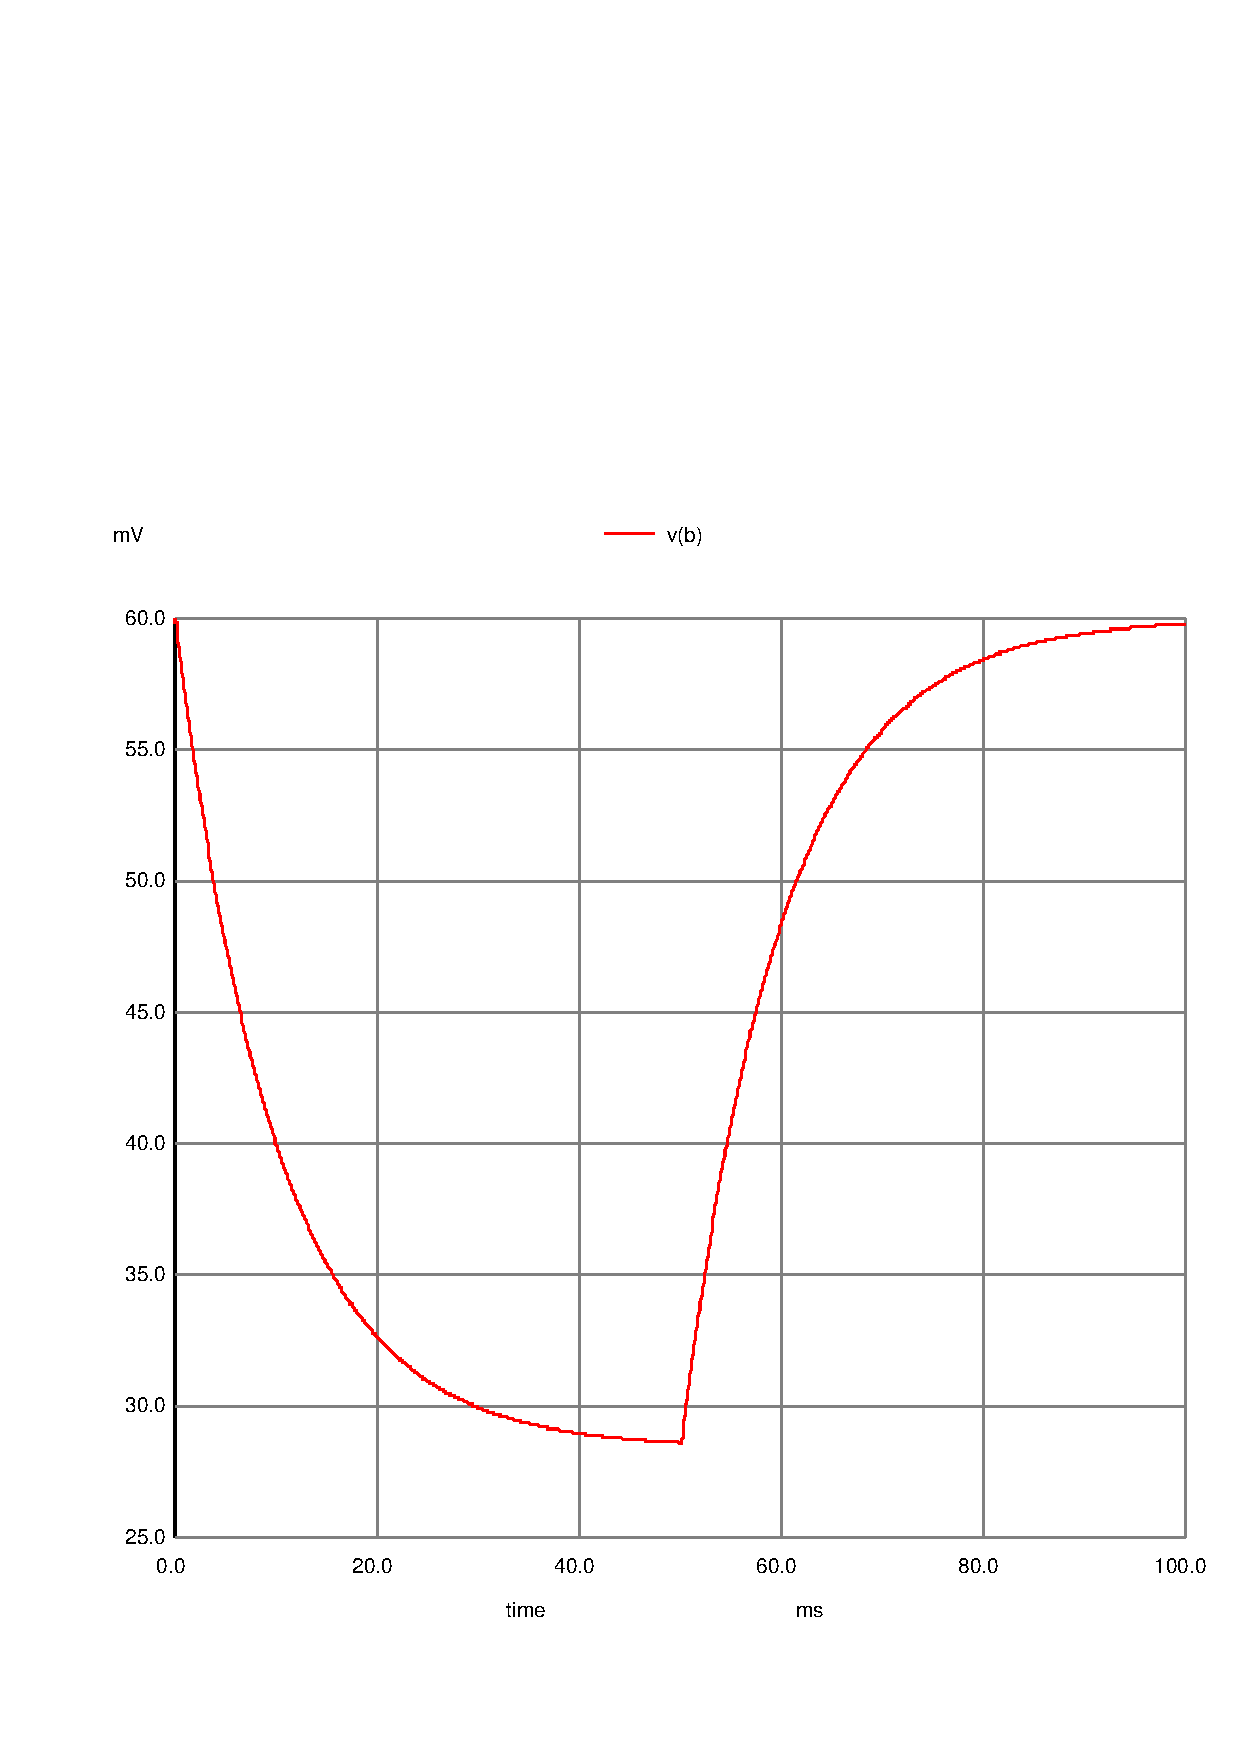
\includegraphics{./plot_1000hz.pdf}.

\end{document}
